% Vorlage fuer Ausarbeitungen
% zum Seminar "Amenable Gruppen"
% im SS 2011
%
%%%%%%%%%%%%%%%%%%%%%%%%%%%%%%%%%%%%%%%%%%%%%%%%%%%%%%%%%%%%%%%%%%%%%%%%%%%%
% Allgemeine Hinweise
% - Halten Sie den LaTeX-Code so uebersichtlich wie moeglich;
%   (La)TeX-Fehlermeldungen sind oft kryptisch -- in einem ordentlich 
%   strukturierten Quellcode lassen sich Fehler leichter finden und 
%   beseitigen
%
%
%%%%%%%%%%%%%%%%%%%%%%%%%%%%%%%%%%%%%%%%%%%%%%%%%%%%%%%%%%%%%%%%%%%%%%%%%%%%
% Jedes LaTeX-Dokument muss eine \documentclass-Deklaration enthalten
%   Diese sorgt fuer das allgemeine Seiten-Layout, das Aussehen der 
%   Ueberschriften etc.
\documentclass[a4paper,twoside,DIV8,10pt]{scrartcl}
  
  %%%%%%%%%%%%%%%%%%%%%%%%%%%%%%%%%%%%%%%%%%%%%%%%%%%%%%%%%%%%%%%%%%%%%%%%%%
  % Einbinden weiterer Pakete
  \usepackage{german}    % fuer die deutschen Trennmuster
  % \usepackage{ngerman} % entsprechend fuer die neue Rechtschreibung
  \usepackage[latin1]{inputenc} % falls Sie Umlaute in den Quellen verwenden wollen
  \usepackage{amsmath}   % enthaelt nuetzliche Makros fuer Mathematik
  \usepackage{amsthm}    % fuer Saetze, Definitionen, Beweise, etc.
  \usepackage{amsfonts}  % spezielle AMS-Mathematik-Fonts
  \usepackage{tikz}      % fuer Graphiken
  \usepackage[headinclude]{scrpage2}  % fuer die Kopfzeilen

  %%%%%%%%%%%%%%%%%%%%%%%%%%%%%%%%%%%%%%%%%%%%%%%%%%%%%%%%%%%%%%%%%%%%%%%%%%
  % Deklaration eigener Mathematik-Makros
  \newcommand{\N}{\ensuremath{\mathbb{N}}}   % natuerliche Zahlen
  \newcommand{\Z}{\ensuremath{\mathbb{Z}}}   % ganze Zahlen
  \newcommand{\Q}{\ensuremath{\mathbb{Q}}}   % rationale Zahlen
  \newcommand{\R}{\ensuremath{\mathbb{R}}}   % reelle Zahlen

  %%%%%%%%%%%%%%%%%%%%%%%%%%%%%%%%%%%%%%%%%%%%%%%%%%%%%%%%%%%%%%%%%%%%%%%%%%
  % Deklaration eigener Satz-/Definitions-/Beweisumgebungen mit amsthm
  \newtheorem{satz}{Satz}[section]
  \newtheorem{lemma}[satz]{Lemma}
  \newtheorem{korollar}[satz]{Korollar}
  \theoremstyle{definition}
  \newtheorem{definition}[satz]{Definition}
  \newtheorem{bemerkung}[satz]{Bemerkung}
  \newtheorem{aufgabe}[satz]{Aufgabe}
  \newenvironment{beweis}%
    {\begin{proof}[Beweis]}
    {\end{proof}}
  \newtheorem{beispiel}[satz]{Beispiel}

  %%%%%%%%%%%%%%%%%%%%%%%%%%%%%%%%%%%%%%%%%%%%%%%%%%%%%%%%%%%%%%%%%%%%%%%%%%
  % Deklaration weiterer Makros
  \renewcommand{\labelitemi}{--}   % aendert die Symbole bei unnumerierten Aufzaehlungen
  \makeatletter                    % Fussnote ohne Symbol
    \def\blfootnote{\xdef\@thefnmark{}\@footnotetext}
  \renewcommand{\sectfont}{\normalfont} % aendert den Font fuer Ueberschriften

  % Seitenlayout
  \renewcommand{\headfont}{\sffamily}  % sans serif Kopfzeilen
  \renewcommand{\pnumfont}{\sffamily}  % sans serif Seitenzahlen
  \automark[section]{section}          % bestimmt den Inhalt von \headmark
  \deftripstyle{myheadings}{\headmark}{}{\pagemark}% Kopfzeile
                           {}{}{}% Fusszeile
  \pagestyle{myheadings}               % aktiviert den neu definierten Seitenstil


  %%%%%%%%%%%%%%%%%%%%%%%%%%%%%%%%%%%%%%%%%%%%%%%%%%%%%%%%%%%%%%%%%%%%%%%%%%
  % Titel der Ausarbeitung
  \author{N.~Imeta (\textsf{nimeta@turbospam.org})}
  \date{42.~Mai 2011}
  \title{Gruppenoperationen%
    \blfootnote{Seminar/Hauptseminar \glqq Amenable Gruppen\grqq, 
      SS~2011, Universit\"at Regensburg}}

%%%%%%%%%%%%%%%%%%%%%%%%%%%%%%%%%%%%%%%%%%%%%%%%%%%%%%%%%%%%%%%%%%%%%%%%%%%%
% Anfang des eigentlichen Dokuments
\begin{document}

  % Titel der Ausarbeitung -- Sie koennen natuerlich auch selbst etwas entwerfen!
  \maketitle

  \begin{abstract}
    \noindent
      
  \end{abstract}

  \section{Der Hauptsatz \"uber Gruppenoperationen}

  Gruppenoperationen werden in den meisten Krankenh\"ausern mittlerweile
  nicht mehr empfohlen. Satz~\ref{hauptsatz} zeigt jedoch, da\ss\
  es immer noch zahlreiche Gruppenoperationen gibt.
  
  \begin{satz}[Hauptsatz \"uber Gruppenoperationen]\label{hauptsatz}
    Zu jeder Menge~$X$ und jeder Gruppe~$G$ gibt es eine
    Grupenoperation von~$G$ auf~$X$.
  \end{satz}
  \begin{beweis}
    Sei $X$ eine Menge und $G$ eine Gruppe. Dann ist
    \begin{align*}
      G \times X & \longrightarrow X \\
      (g,x)      & \longmapsto     x
    \end{align*}
    eine Operation von~$G$ auf~$X$.
  \end{beweis}

  Auf dieselbe Art und Weise lassen sich nat\"urlich auch
  Definitionen, Lemmata und Korollare etc.\ mit \LaTeX\ darstellen.

  Bei Fragen zu \LaTeX\ ist der \emph{\LaTeX\ Companion}~\cite{companion} 
  eine gro\ss e Hilfe; Sie k\"onnen Sich aber auch gerne an Clara
  L\"oh (\textsf{clara.loeh@mathematik.uni-regensburg.de}) oder an 
  Matthias Blank (\textsf{matthias.blank@mathematik.uni-regensburg.de}) 
  wenden.

  \section{Beispiele}

  \begin{beispiel}
    \hfil
    \begin{itemize}
      \item Hier ein Beispiel 
      \item \dots und noch eins
      \item \dots und noch eins
      \item \dots und noch eins
    \end{itemize}
  \end{beispiel}

  \begin{aufgabe}
    Vergessen Sie nicht, ein paar Aufgaben einzustreuen, an denen die
    Teilnehmer nochmal ihre Kenntnisse \"uberpr\"ufen k\"onnen.
  \end{aufgabe}

  \begin{beispiel}
    \hfil
    \begin{enumerate}
      \item Es gibt auch Beispiele, \dots
      \item \dots die numeriert sind.
    \end{enumerate}
  \end{beispiel}

  Graphiken lassen sich z.B.\ mit \emph{TikZ}~\cite{tantau} erstellen;
  Abbildung~\ref{fig:hausvomnikolaus} zeigt eine Illustration des \glqq
  Hauses vom Nikolaus\grqq, d.h.\ des Graphen~$(V,E)$ mit Knotenmenge~$V
  = \{1,\dots,5\}$ und Kantenmenge
  \begin{align*}
    E & := \bigl\{ \{1,2\}
                 , \{1,5\}
                 , \{2,3\}
                 , \{2,4\}
                 , \{2,5\}
                 , \{3,4\}
                 , \{3,5\}
                 , \{4,5\}
           \bigr\}.
  \end{align*}

  \begin{figure}
    \begin{center}
      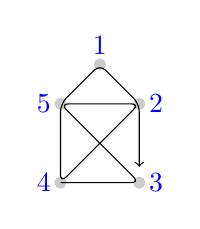
\begin{tikzpicture}
         \begin{scope}[color=black!20]
           \draw[fill] (0,0) circle (2pt);
           \draw[fill] (1,0) circle (2pt);
           \draw[fill] (0,1) circle (2pt);
           \draw[fill] (0.5,1.5) circle (2pt);
           \draw[fill] (1,1) circle (2pt);
         \end{scope}
         \begin{scope}[color=blue]
           \draw (0.5,1.5) node[above] {$1$};
           \draw (1,1) node[right] {$2$};
           \draw (1,0) node[right] {$3$};
           \draw (0,0) node[left] {$4$};
           \draw (0,1) node[left] {$5$};
         \end{scope}
         \draw[->,rounded corners=0.1cm]
            (0,0) -- (1,0) -- (0,1) -- (1,1) -- (0,0)
         -- (0,1) -- (0.5,1.5) -- (1,1) -- (1,0.2);
      \end{tikzpicture}
    \end{center}
    \caption{Das Haus vom Nikolaus}
    \label{fig:hausvomnikolaus}
  \end{figure}

%%%%%%%%%%%%%%%%%%%%%%%%%%%%%%%%%%%%%%%%%%%%%%%%%%%%%%%%%%%%%%%%%%%%%%%%%%%%
% Literaturverzeichnis
% - Der Einfachheit halber sind hier bereits alle Quellen eingetragen, 
%   die im Seminarprogramm auftreten
% - Bitte entfernen Sie alle Quellen, die Sie nicht in Ihrem Handout 
%   zitieren
% - Umgekehrt muessen Sie natuerlich, wenn Sie weitere Literatur
%   zitieren wollen, die entsprechenden Quellen hier einfuegen; 
%   hierbei kann www.ams.org/mathscinet helfen, die noetigen 
%   Informationen zu den Quellen zu sammeln
\begin{thebibliography}{99}

    \bibitem{beutelspacher} A.~Beutelspacher. \emph{Das ist o.B.d.A.\
        trivial!}, neunte Auflage, Vie\-weg$+$Teub\-ner, 2009.

   \bibitem{bridsonhaefliger} 
      M.R.~Bridson, A.~Haefliger. 
      \emph{Metric Spaces of Non-positive Curvature},
      Band~319 der \emph{Grundlehren der Mathematischen
        Wissenschaften}, Springer, 1999.

  \bibitem{csc} T.~Ceccherini-Silberstein,
    M.~Coornaert. \emph{Cellular Automata and Groups}, Springer
    Monographs in Mathematics, Springer, 2010.

   \bibitem{delaharpe} P.~de~la~Harpe.
      \emph{Topics in Geometric Group Theory}, 
      Chicago University Press, 2000.


    \bibitem{hhm} J.M.~Harris, J.L.~Hirst,
      M.J.~Mossinghoff. \emph{Combinatorics and Graph Theory}, zweite
      Auflage, Undergraduate Texts in Mathematics, Springer, 2008.


    \bibitem{jacobs} K.~Jacobs. \emph{Einf\"uhrung in die Kombinatorik},
      de~Gruyter, 1983.

    \bibitem{ggt} C.~L\"oh. \emph{Geometric group theory, an
        introduction}, Skript zur Vorlesung \glqq Geometrische
      Gruppentheorie\grqq\ im WS~2010/11, Universit\"at Regensburg,\\ 
      \textsf{http://www.mathematik.uni-regensburg.de/loeh/teaching/ggt\_ws1011/lecture\_notes.pdf}

    \bibitem{companion} F.~Mittelbach, M.~Goossens, J.~Braams,
      D.~Carlisle, C.~Rowley. \emph{The \LaTeX\ Companion}, zweite
      Auflage, Addison-Wesley, 2004.

   \bibitem{paterson}
      A.L.T.~Paterson. \emph{Amenability}, 
      volume~29 of~\emph{Mathematical Surveys and Mono\-graphs}, American
      Mathematical Society, 1988.

    \bibitem{runde}
      V.~Runde, \emph{Amenability}, volume~1774 of~\emph{Springer
        Lecture Notes in Mathematics}, Springer, 2002.

   \bibitem{tantau} 
        T.~Tantau. \emph{The {\normalfont Ti\textit{k}Z} and
          {\normalfont PGF} Packages}, 
        \\
        \textsf{http://www.ctan.org/tex-archive/graphics/pgf/base/doc/generic/pgf/pgfmanual.pdf} 

   \bibitem{whyte} K.~Whyte. Amenability, bi-Lipschitz equivalence,
      and the von Neumann conjecture, \emph{Duke Math.~J.}~99, No.~1, 
      S.~93--112, 1999.

\end{thebibliography}

%%%%%%%%%%%%%%%%%%%%%%%%%%%%%%%%%%%%%%%%%%%%%%%%%%%%%%%%%%%%%%%%%%%%%%%%%%%%
% Ende des Dokuments -- alles, was nach dieser Zeile steht, wird 
% von LaTeX ignoriert!
\end{document}